
\chapter{Le modele standard de la cosmologie moderne}
 \label{ch:introduction_physique}

Cette thèse s'inscrit dans le cadre du modèle standard de la cosmologie.
Ce modèle, aussi appelé modèle $\Lambda$CDM, considère un Univers en expansion et composé essentiellement d'énergie noire ($\Lambda$) et de matière noire froide (Cold Dark Matter). 
Ce chapitre a pour objectif de présenter les grandes lignes de ce modèle.

\section{Émergence de l'idée d'un Univers non statique}

%découverte des galaxies\\
%découverte de l'expansion de l'univers

%\subsection{Cadre théorique}

L'idée d'un Univers non statique a pris forme dans le début du XXème siècle suite à deux événements majeurs.
D'un coté l'élaboration de la théorie de la relativité générale d'Einstein en 1915 a permis la mise en place d'un cadre théorique propice.
%La notion d'un univers non statique a ete introduite par Einstein en 1917 en rapport avec ses travaux sur le relativité générale. 
D'un autre coté, plus d'une décennie plus tard les observations de Hubble ont confirmé l'expansion de l'Univers.

\subsection{Les observations de Hubble}

Entre 1923 et 1929 Hubble observe deux phénomènes qui vont mener à une redéfinition de notre notion de cosmologie.
Il bénéficie à l'époque de l'accès au plus puissant télescope du monde (le télescope Hooker du mont Wilson).
Cet instrument lui a permis d'observer que des nébuleuses situées hors de notre galaxie présentent des caractéristiques identiques à des systèmes d'étoiles \citep{1926ApJ....63..236H}.
Il en déduit qu'il existe d'autres galaxies que notre Voie Lactée (voir figure \ref{fig:hubbl_deep_field}).

%Avec les moyens observationnels dont nous disposons aujourd'hui l’existence d'un grand nombre de galaxies en dehors de notre voie lactée est bien établie.
%Le "Hubble Ultra Deep Field"  (voir figure \ref{fig:hubbl_deep_field}) une image prise en 2004 et publiée en 2006 \citep{1538-3881-132-5-1729} montre un grand nombre de galaxies dans une portion réduite du ciel.
%On estime aujourd'hui le nombre de galaxies à $\approx 2 \cdot 10^{11}$ dans l'Univers observable.

\begin{figure}
        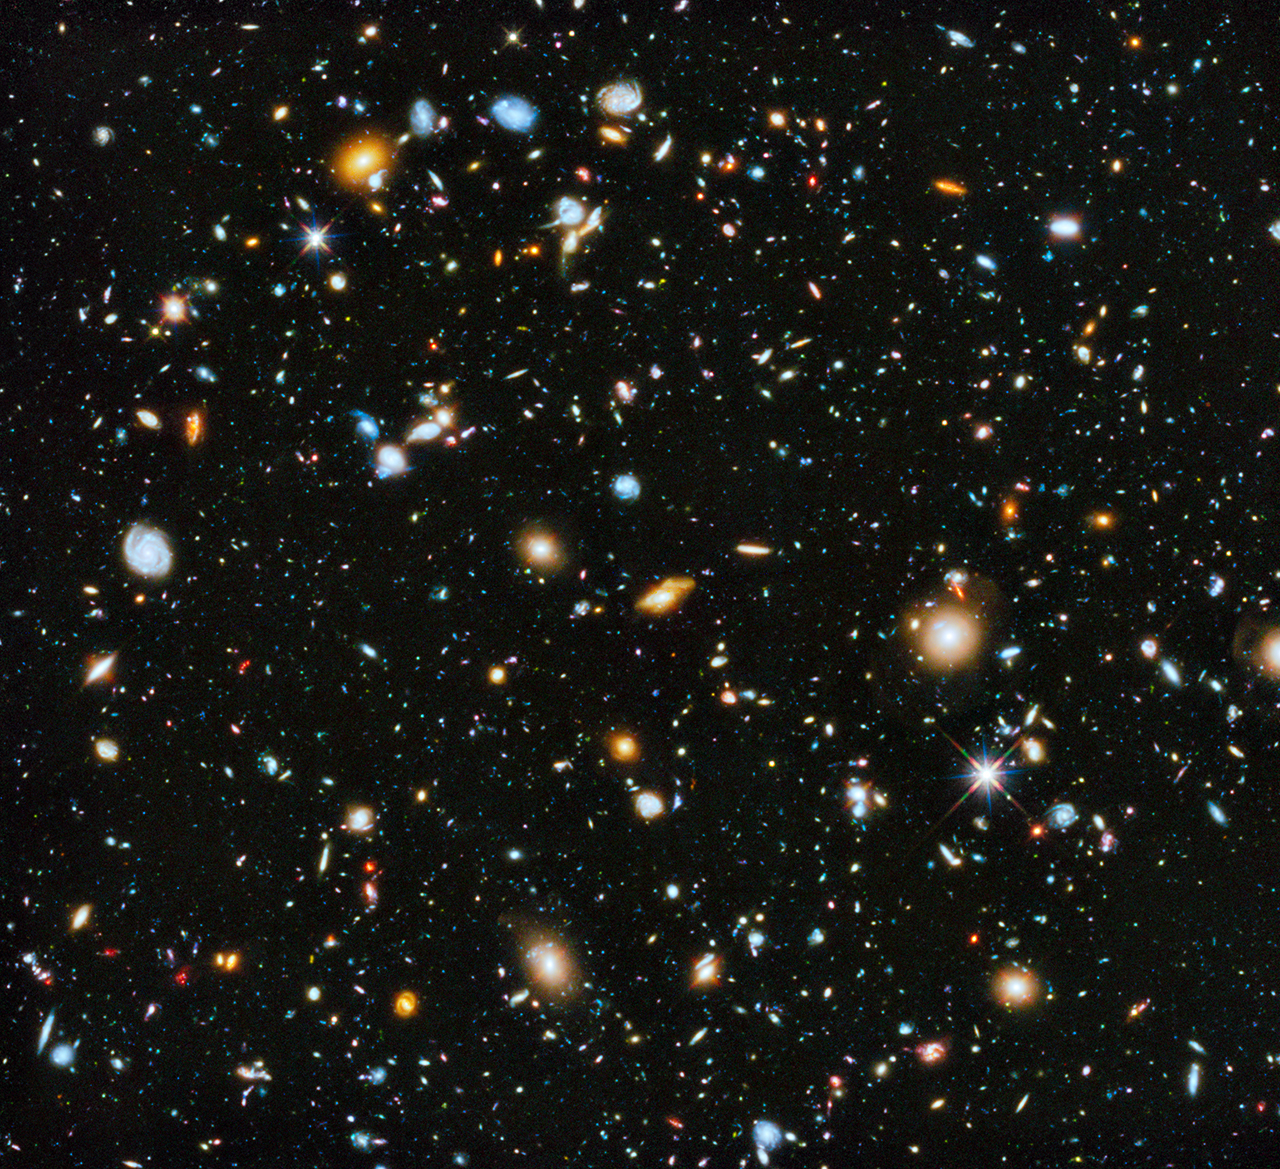
\includegraphics[width=.9\linewidth]{img/01/hudf.jpeg} 
        \caption[Hubble Ultra Deep Field]{Hubble Ultra Deep Field \citep{1538-3881-132-5-1729}.
        %2014.
        %Image NASA.
		En 1926 E. Hubble observe pour la première fois qu'il existe d'autre galaxies.
		Leur nombre est estimé aujourd'hui à $\approx 2 \cdot 10^{11}$ dans l'Univers observable.
 		\label{fig:hubbl_deep_field}}
\end{figure}

\subsection{La loi de Hubble}
\cite{1929CoMtW...3...23H} observe également une relation entre la distance de ces nouvelles galaxies et leurs spectres lumineux.
Plus une galaxie est éloignée de l'observateur, plus son spectre est décalé vers le rouge.
%Ce redshift noté $z$ est une notion qui sera beaucoup utilisée par la suite car nous verrons dans la prochaine section qu'il existe un lien direct entre âge de l'univers et redshift.
%Il interpréta ce décalage comme un effet Doppler et montra que ces galaxies s'éloignent de l'observateur avec une vitesse radiale directement proportionnelle à leur distance.
%Cette corrélation entre la distance et le décalage vers le rouge observé est aujourd'hui bien établie (voir figure \ref{fig:hubble_law}).
%Une série d'observations récentes est présenté sur la .
%
%\begin{figure}
%        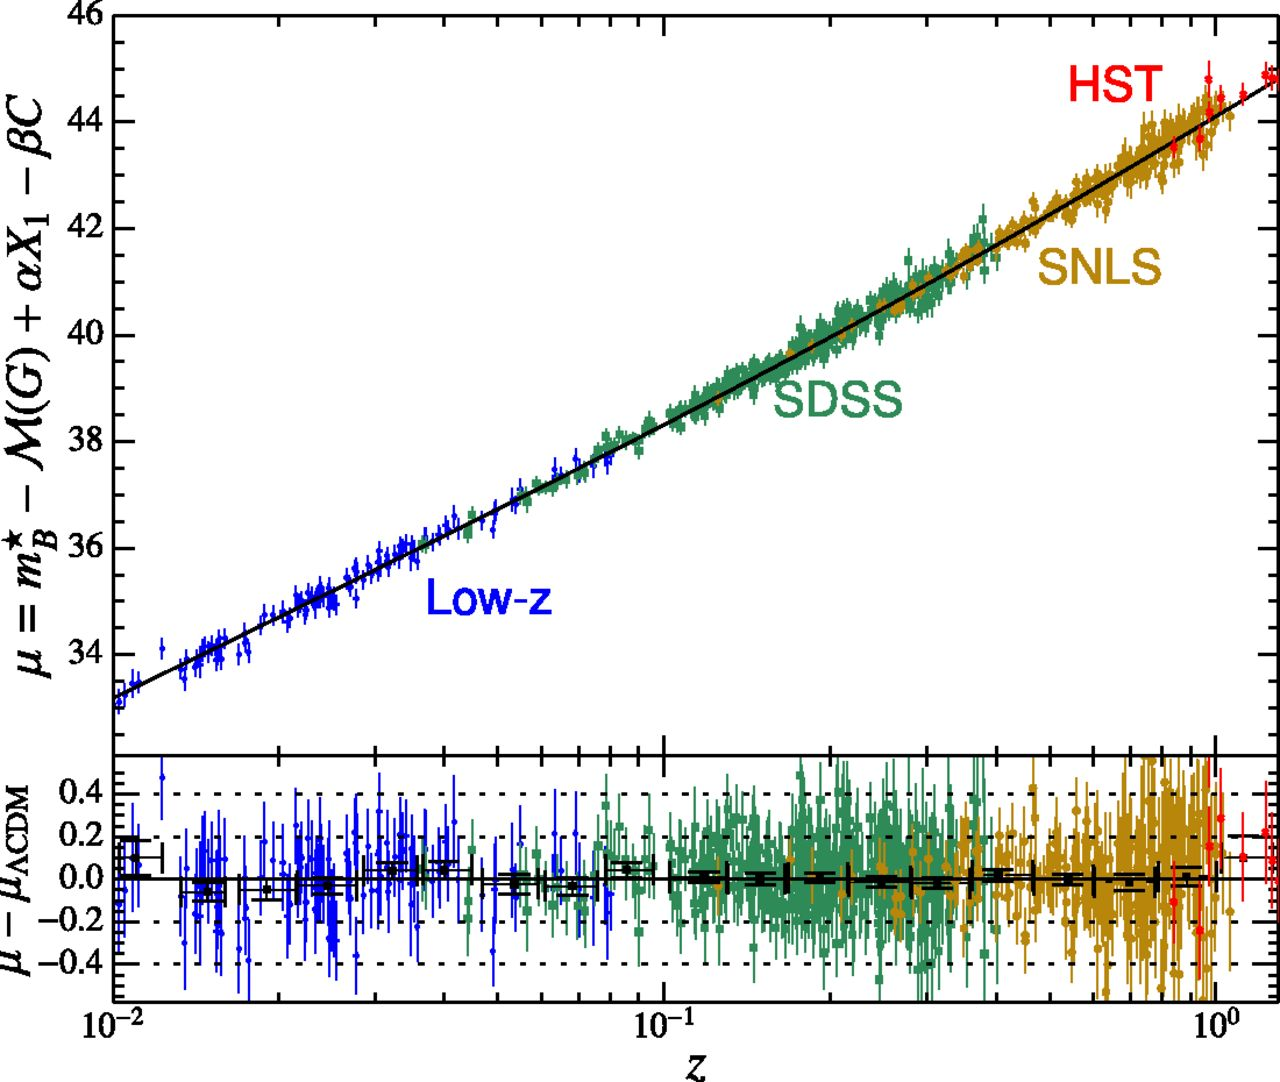
\includegraphics[width=.9\linewidth]{img/01/hubble_law.jpg} 
%        \caption[Loi de Hubble]{Loi de Hubble à partir d'observations actuelles. 
%        Figure extraite de \citep{2015PNAS..112.3173B}.
%%http://www.pnas.org/content/112/11/3173/F2.expansion.html
%%        Image ESO
%        }
% 		\label{fig:hubble_law}
%\end{figure}

La loi de Hubble est la relation entre la distance d'une galaxie $D$ et sa vitesse radiale d'éloignement $V$ : %est aujourd'hui appelée  et peux être résumé par :

\begin{equation}
V = H_0 D,
\end{equation}
où la constante de Hubble est aujourd'hui estimée à $H_0 = 67$ $\mathrm{ \left[ km.s^{-1}.Mpc^{-1} \right ] }$ \citep{planck_collaboration_planck_2016}.

%Conventionnellement, le sous script $0$ désigne le fait que la valeur de la variable qui lui est associé est celle prise aujourd'hui.
%Cette distinction est nécessaire car malgré son nom, la valeur de la constante de Hubble n'est pas constante dans le temps.
D'une manière plus générale la constante de Hubble représente le taux de variation relative de la distance entre deux points.
Elle s'exprime sous la forme:
\begin{equation}
H=\frac{1}{a} \frac{da}{dt} = \frac{\dot{a}}{a},
\end{equation}

où $a = a_{(t)}$ est le facteur d'expansion.
$a_0=1$ représente par définition la valeur de $a$ prise aujourd'hui.

%Comme la longueur d'une onde lumineuse est aussi impactée par l'expansion, 
Le redshift, s'exprime en fonction du facteur d'expansion de la manière suivante:
\begin{equation}
z= \frac{1}{a}-1
\end{equation}

\subsection{Équations de Friedmann}
\label{sec:friedman}

Les observations de Hubble ont permis de confirmer ce qui avait été pressenti par \cite{1916AnP...354..769E} plus d'une décennie plus tôt, lorsqu'il introduisit théoriquement le concept d'expansion de l'Univers. 
La théorie de la relativité générale introduit la célèbre equation de champ décrivant le lien entre densité d'énergie et déformation de l'espace-temps:

%Equation d'Einstein 
%http://cdsads.u-strasbg.fr/abs/1915SPAW.......844E
\begin{equation}
R_{\mu\nu} - \frac{1}{2} g_{\mu\nu}R + \Lambda g_{\mu\nu}  = \kappa T_{\mu\nu}.
\label{eq:einstein}
\end{equation} 

Dans cette équation apparaît le terme $\Lambda$ (de $\Lambda$CDM), appelée \textit{constante cosmologique}, et également :
%Cette constante représente mathématiquement le fait que l'espace-temps peut être en expansion ou en contraction.
$R_{\mu \nu}$ le tenseur de Ricci, $R$ la courbure scalaire, $g_{\mu \nu}$ le tenseur métrique, $T_{\mu \nu }$ le tenseur énergie-impulsion et $\kappa$ la constante d'Einstein.

%Metrique de Friedmann-Lemaître-Robertson-Walker (FLRW)

Quelques années plus tard, Alexandre Friedmann entreprend de trouver des solutions exactes à l'équation d'Einstein en l'appliquant à un Univers homogène et isotrope \citep{1922ZPhy...10..377F}.
Il arrive à ce système d'équations indépendantes permettant de modéliser l'Univers dans son ensemble :

%Recriture de l equation d'Einstein en considerant un univers homogene et isotrope.
% 
%Alexandre Friedmann Über die Krümmung des Raumes, Zeitschrift für Physik 10, 377-386 (1922). 
%Première écriture des équations de Friedmann, dans le cas d'une coubure spatiale positive. http://cdsads.u-strasbg.fr/abs/1922ZPhy...10..377F 
%
%(de) Alexandre Friedmann, Über die Möglichkeit einer Welt mit konstanter negativer Krümmung des Raumes, Zeitschrift für Physik 21 326–332 (1924). 
%Écriture des équations de Friedmann dans le cas d'une courbure spatiale négative. 
% 
%univers de Friedmann-Lemaître-Robertson-Walker  
%http://dictionnaire.sensagent.leparisien.fr/%C3%89quations%20de%20Friedmann/fr-fr/
 
%Équations de Friedmann : 

\begin{equation}
3 \left( \frac{H^2}{c^2} +\frac{K}{a^2} \right) = \frac{8 \pi G }{c^2} \rho
\label{eq:friedman1}
\end{equation}

\begin{equation}
-2 \frac{ \dot{H}}{c^2} -3 \frac{H^2}{c^2} -\frac{K}{a^2} = \frac{8 \pi G }{c^4 P}
\label{eq:friedman2}
\end{equation}

L'équation \ref{eq:friedman1} relie le taux d'expansion $H$, la courbure spatiale $K$ et le facteur d'échelle $a$ à la densité d'énergie $\rho$.
L'équation \ref{eq:friedman2} relie la pression $P$ à la dérivée temporelle du taux d'expansion.
  
En manipulant l'équation \ref{eq:friedman1} il est possible de montrer que :
% cf 
% http://dictionnaire.sensagent.leparisien.fr/%C3%89quations%20de%20Friedmann/fr-fr/
% https://en.wikipedia.org/wiki/Friedmann_equations
% pour la demonstration

%TODO introduire les differents fluides cosmologiques

\begin{equation}
H = \frac{\dot{a}}{a} = H_0 \sqrt{ \Omega_{r,0} a^{-4} +  \Omega_{M,0} a^{-3} + \Omega_{K,0}a^{-2} + \Omega_{\Lambda,0}  } 
\label{eq:scale_t}
\end{equation}


\begin{figure}
        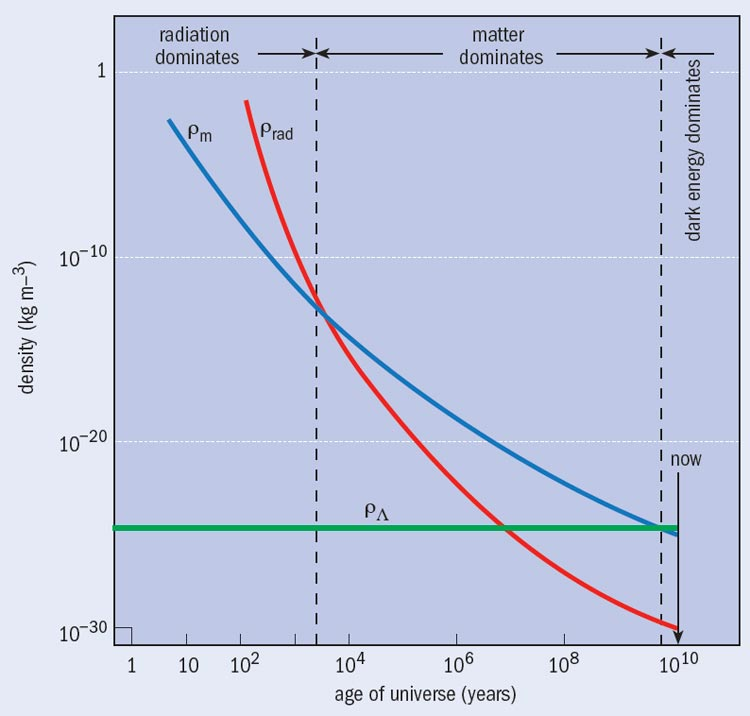
\includegraphics[width=.9\linewidth]{img/01/dark4.jpg} 
        \caption[Densités d'énergies]{Importance respective des différentes densité d'énergie en fonction de l'age de l'Univers (et donc de sa taille). Image extraite de \citep{2005univ.book.....F}
 		\label{fig:cosmoparamt} }
\end{figure}


où les paramètres $\Omega_{i,0}$ représentent la densité d'énergie associée aux différents constituants, 
\begin{equation}
 \Omega_{i,0} = \frac{\rho_{i,0}}{\rho_{c,0}},
 \end{equation}

en fonction de la densité critique de l'Univers:

\begin{equation}
\rho_{c,0} = \frac{3H_0^2}{8\pi G}
 \end{equation}
Nous verrons dans la partie dédiée à la détermination des paramètres cosmologiques (cf Sec \ref{cosmoparam}) que les mesures actuelles sont en faveur d'un Univers plat (sans courbure).
Ce qui s'exprime par $\Omega_{K,0} = 0$ et $\Omega_{\lambda,0} +  \Omega_{M,0} + \Omega_{r,0} =1$.
La valeur de $\rho_c$ est déterminée avec l'équation \ref{eq:friedman1}, en considérant un Univers plat et sans constante cosmologique ($\Lambda=0$).

\paragraph{$\Omega_{M,0}$} est le paramètre de densité d'énergie associée à la matière. % (matière noire que nous introduiront dans la suite et la matière baryonique)
Par simple effet de dilution, cette densité décroît avec le cube du facteur d'expansion.
Un Univers dominée par cette énergie est nommé "Univers poussière".
%C'est le cas actuellement.

\paragraph{$\Omega_{r,0}$} représente le paramètre de densité d'énergie relativiste (par exemple les photons).
La densité de photon décroît avec le cube du facteur d'expansion, mais du fait de l'allongement de la longueur d'onde avec $a$, la densité d'énergie associée au rayonnement décroît avec la puissance $4$ de $a$.
Un Univers dominée par cette énergie est nommé "Univers lumière".
%Cette approximation est valable pour un Univers majoritairement remplis de matière relativiste.
%C'était le cas avant l’émission du fond diffus cosmologique.

\paragraph{$\Omega_{\Lambda,0}$} est le paramètre de densité d’énergie du vide.
Cette énergie est associée à la constante cosmologique et à l'accélération de l'expansion de l'Univers et sa densité est constante dans le temps.

\paragraph{$\Omega_{K,0}$} est le paramètre de densité de courbure spatiale ou la densité d'énergie associée à la courbure de l'espace.
Selon l’équation \ref{eq:einstein}, l'énergie peut courber l'espace, mais si l'espace possède une courbure intrinsèque, elle est équivalente à une densité d'énergie.
\begin{equation}
\Omega_{K,0} = 1 - \Omega_{r,0} - \Omega_{M,0} - \Omega_{\lambda,0} 
\end{equation}

Comme ces densités d'énergies sont liées au facteur d'expansion, celles-ci évoluent avec le temps (cf Fig. \ref{fig:cosmoparamt}) et dominent à différentes époques.
Lors de la réionisation, le bilan énergétique de l'Univers était dominé par la matière.

\begin{figure}
        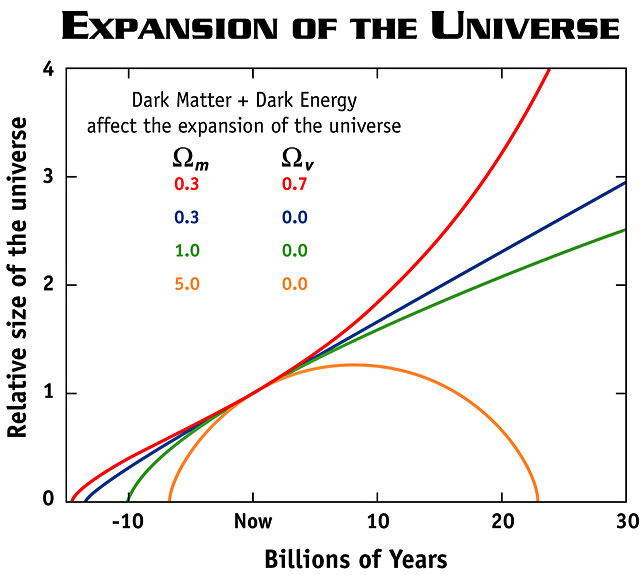
\includegraphics[width=.9\linewidth]{img/01/scale_t.jpg} 
        \caption[Taille de l'Univers]{Taille de l'Univers en fonction du temps pour différents paramètres cosmologiques.
		Image \href{https://map.gsfc.nasa.gov/universe/bb_concepts_exp.html}{NASA/WMAP Science Team}.
 		\label{fig:scale_t}}
\end{figure}

En intégrant l’équation \ref{eq:scale_t}, il est possible de déterminer l'évolution de la taille de l'Univers en fonction de la densité respectives de ses différents constituants.
La figure \ref{fig:scale_t} présente quelques évolutions possibles.
%Toutes les courbes passent par le point (Now,1) car par définition $a_0 = 1$.
%TODO expliquer cette histoire de tangente
%Toutes les courbes ont la même tangente au point (Now,1) du fait que $\Omega_{K,0}=0$
%TODO dire que nous somme la courbe rouge
Nous observons ici que la valeur des paramètres cosmologique contraint l'age actuel de l'Univers (le point où la courbe passe l'axe horizontal).
%La valeur des paramètres contraint aussi l'avenir de l'Univers.
%Par exemple, la courbe orange représente un Univers dit fermé.
%Ce type d'Univers est voué à s'effondrer sur lui même à cause de la gravité de la matière qu'il contient.
%A l'inverse, la courbe rouge représente un Univers dit ouvert.
%La gravitation n'est pas suffisante pour contrer l'expansion, et ce type d'Univers est voué a grandir indéfiniment.
%TODO dire que nous somme dans la courbe rouge
%\cite{2003PhT....56d..53P}

Le scénario actuellement admis est en faveur d'un Univers en accélération (courbe rouge).
L'accélération de l'expansion de l'univers a été découverte à la fin du XXème siècle par 2 équipes simultanément, chacune ayant reçue le prix Nobel en 2011 :
\begin{itemize}
\item  High-Z supernovae search team \citep{1998AJ....116.1009R} %http://cdsads.u-strasbg.fr/abs/1998AJ....116.1009R
\item  Supernova Cosmology Project \citep{1999ApJ...517..565P} % http://cdsads.u-strasbg.fr/abs/1999ApJ...517..565P
\end{itemize}

%\subsection{Énergie noire}
%\label{sec:dark_egy}
%
%%Dans un Univers, ou seule la gravité agit a grandes échelles, l'expansion ne peux que décélérer.
%
%Si nous avons vu que la taille de l'Univers évolue avec le temps, il reste la question de l'accélération de cette évolution.
%Si l'on considère que l'univers s'étend suite à une impulsion initiale (cf section \ref{sec:BB}), et que la gravité est la seule force qui agit à grande échelle, l'expansion devrait décélérée.
%%En effet comme la gravité est une force purement attractive, elle agit comme un ressort qui devrait ramener toute la masse à l'origine (scénario de la courbe orange sur la figure \ref{fig:scale_t}, ou la courbe retombe sur l'axe horizontal signifiant que la taille de l'univers tend à nouveau vers zero).
%Or ce n'est pas ce qui est observé: l'accélération de l'expansion de l'univers a été découverte a la fin du XXème siècle par 2 équipes simultanément, chacune aillant reçu le prix Nobel en 2011 :
%\begin{itemize}
%\item  High-Z supernovae search team \citep{1998AJ....116.1009R} %http://cdsads.u-strasbg.fr/abs/1998AJ....116.1009R
%\item  Supernova Cosmology Project \citep{1999ApJ...517..565P} % http://cdsads.u-strasbg.fr/abs/1999ApJ...517..565P
%\end{itemize}
%
%L'accélération de l'expansion de l'Univers pose un problème majeur.
%Il est établi depuis les travaux de Newton que pour accélérer une masse une force est nécessaire.
%Or nous ne disposons actuellement d'aucune théorie permettant d'expliquer cette force répulsive.
%Il a fallu seulement quelques mois après cette découverte pour qu’apparaisse pour la première fois la mention d'énergie noire \citep{1999PhRvD..60h1301H}.
%
%%échelle gigaparsec\\
%%Facteur d'expansion


\clearpage
\section{Le modèle du Big-bang}
\label{sec:BB}
%le big bang\\
%l'inflation\\
%la nucléosynthèse\\
%le CMB\\
%la reionization

Une fois établi que les galaxies s'éloignent de nous dans toutes les directions, un constat s'impose : en remontant le temps elles devaient être plus proches les unes des autres, et en poussant ce constat à l’extrême, à un certain instant dans l'histoire de l'Univers, toute la matière était extrêmement dense.
\cite{1927ASSB...47...49L} propose une théorie de l'atome primitif.
Cette singularité a été baptisée Big-bang et donne son nom au modèle cosmologique actuel.

%\subsection{Température de l'Univers}
%
%Il existe un lien direct entre la taille de l'Univers et sa température.
%Dans la conception actuelle de l'Univers, celui ci est par définition l'ensemble de ce qui existe, il ne lui est pas possible d'échanger de l’énergie avec l’extérieur : c'est donc un système isolé adiabatique.
%Or, la thermodynamique nous dit qu'il existe une relation entre le volume et la température d'un tel système : la température (la densité d'énergie interne) diminue au fur et à mesure que l'Univers se dilate.
%Plus l'on se rapproche temporellement du BigBang, plus l'Univers est dense et chaud.

\subsection{Nucléosynthèse primordiale}
\label{sec:nucleosynthese_primordiale}
%Dans le modèle du Big Bang, le début de l'Univers est suivis par une phase d'expansion rapide appelé inflation.
Après le Big-bang, l'Univers est suffisamment chaud pour présenter une soupe de particules élémentaires (quarks, gluons, leptons) qui vont former en se refroidissant les premiers protons et neutrons, qui vont à leur tour s'assembler pour former les premiers noyaux atomiques.
La théorie de la nucléosynthèse primordiale a été présentée par \citep{PhysRev.73.803} dans un article surnommé $\alpha \beta \gamma$ en référence aux initiales des noms de ses auteurs.
Cette théorie permet d'expliquer avec précision l'abondance observée des différents atomes présents dans l'Univers.
Il est aujourd'hui admis que l'abondance en masse de l'Univers est : 

\begin{itemize}
\item 73,9\% d’hydrogène,
\item 24\% d’hélium,
\item et 2.1\% de l'intégralité des autres éléments du tableau périodique (nous nommerons ces éléments "métaux" par convention).
\end{itemize}

L'hydrogène est largement majoritaire et l'hélium et les métaux seront négligés dans la suite de cette étude.

\subsection{Le fond diffus cosmologique}
\label{sec:CMB}

Tôt dans l'histoire de l'Univers, les noyaux atomiques sont découplés des électrons et l'Univers est dans un état ionisé. % correspondant à un plasma proche de celui que l'on peut trouver dans une étoile.
Il faudra attendre $\approx 380 000$ ans pour que la température diminue suffisamment pour permettre l'apparition des premiers atomes neutres.
Cette période est appelée "époque de recombinaison" (voir \cite{2009AN....330..657S} pour plus d'informations sur le sujet) et a donnée lieu à l'émission du fond diffus cosmologique ou \ac{CMB}.
Durant cette transition, l'Univers a connu un changement d'état majeur puisque celui-ci est passé d'un état globalement ionisé à un état globalement neutre.
%Comme nous venons de le voir, l’émission du \ac{CMB} marque la transition entre deux états distincts de l'Univers.
Robert Herman et Ralph Alpher ont été les premiers à proposer l’existence du \ac{CMB} en 1948 avant même sa découverte.
%Le \ac{CMB} étant la plus ancienne lumière que nous pouvons observer, il contient actuellement l'information que nous pouvons obtenir sur l'état de l'Univers lorsqu'il était le plus jeune possible.
%
%\subsection{Surface de dernière diffusion}
%
%En raison du grand nombre d'électrons libres avant la recombinaison, la lumière était soumise à un grand nombre de diffusions.
%À la manière de la surface d'une étoile, où nous ne voyons que les photons qui ont pu s’échapper de celle ci et non ceux qui ont été émis en son centre, nous ne pouvons pas observer de lumière émise avant le \ac{CMB}.
%Le \ac{CMB} étant la plus ancienne lumière que nous pouvons observer, il contient actuellement l'information que nous pouvons obtenir sur l'état de l'Univers lorsqu'il était le plus jeune possible.

%La quête de l'état de l'Univers à ses début a commencé de manière fortuite en 1964 quand Penzias et Willson ont observé, lors de travaux sur un nouveau type d’antenne radio, un signal radio inexpliqué.
%Ce signal était constant et extrêmement homogène. 
%(l'anisotropie du CMB est remis en cause recement 
%http://www.ca-se-passe-la-haut.fr/2013/09/lanisotropie-du-fond-diffus-cosmologique.html)
Penzias et Willson ont observé le \ac{CMB} en 1964 et obtiennent le prix Nobel en 1978 pour la \cite{PenziasWilsonNobel}.
Cette observation constitue un argument de poids en faveur de la théorie du Big-bang et une série de missions spatiales lui ont été consacrées.
%dans le but d'améliorer les mesures faites sur le \ac{CMB}.

\begin{itemize}
\item le satellite COBE (COsmic Background Explorer) en 1989
\item le satellite WMAP (Wilkinson Microwave Anisotropy Probe) en 2001
\item le satellite Planck en 2009
\end{itemize}

%\subsection{Température}
%Le \ac{CMB} se présente sous la forme du corps noir à une température de T=2.73°K.
%La figure \ref{fig:cmb_thermal_spectrum} compare le spectre thermique observé à celui d'un corps noir théorique. 
%La correspondance est presque parfaite.
%
%Le \ac{CMB} a été émis lorsque l'Univers était à une température de $T \approx 3000$ K.
%Le signal reçu est donc redshifté d'un facteur $z\approx1100$ par rapport à celui émis lors de la recombinaison.
%
%\begin{figure}[htbp]
%        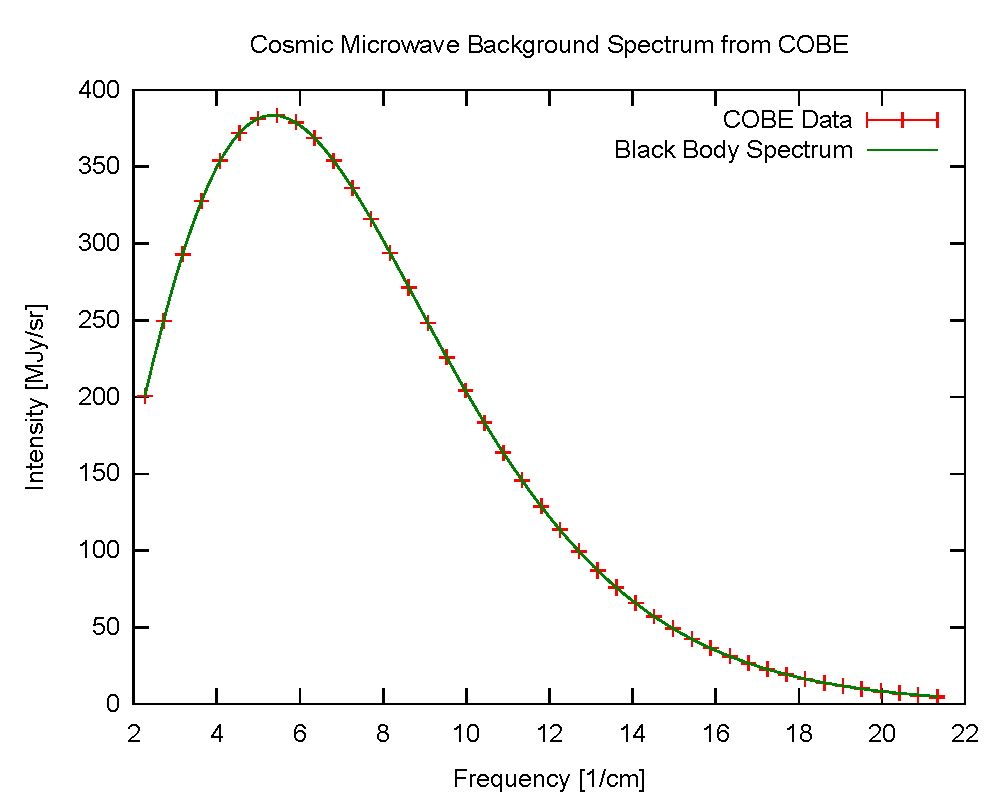
\includegraphics[width=.95\linewidth]{img/01/Cmbr.pdf} 
%        \caption[Température CMB]{Spectre thermique du \ac{CMB} vue par le satellite Cosmic Background Explorer (COBE). 
%        Image Wikipédia
% 		\label{fig:cmb_thermal_spectrum}}
%\end{figure}

Lors de sa découverte, le \ac{CMB} était considéré comme uniforme mais John C. Mather et George F. Smoot ont conjointement obtenus le prix Nobel de physique en 2006 pour la \cite{CMBanisotropiesNobel} grâce aux observations réalisées par le satellite  COBE.
Ce léger défaut d'uniformité (de l'ordre de $10^{-5}$ en relatif) nous renseigne sur l’état de l'Univers au moment de son émission.
Par la suite, les satellites WMAP et Planck ont grandement amélioré la précision des mesures des anisotropies du fond diffus (Fig. \ref{fig:cmb}).

\begin{figure}
%        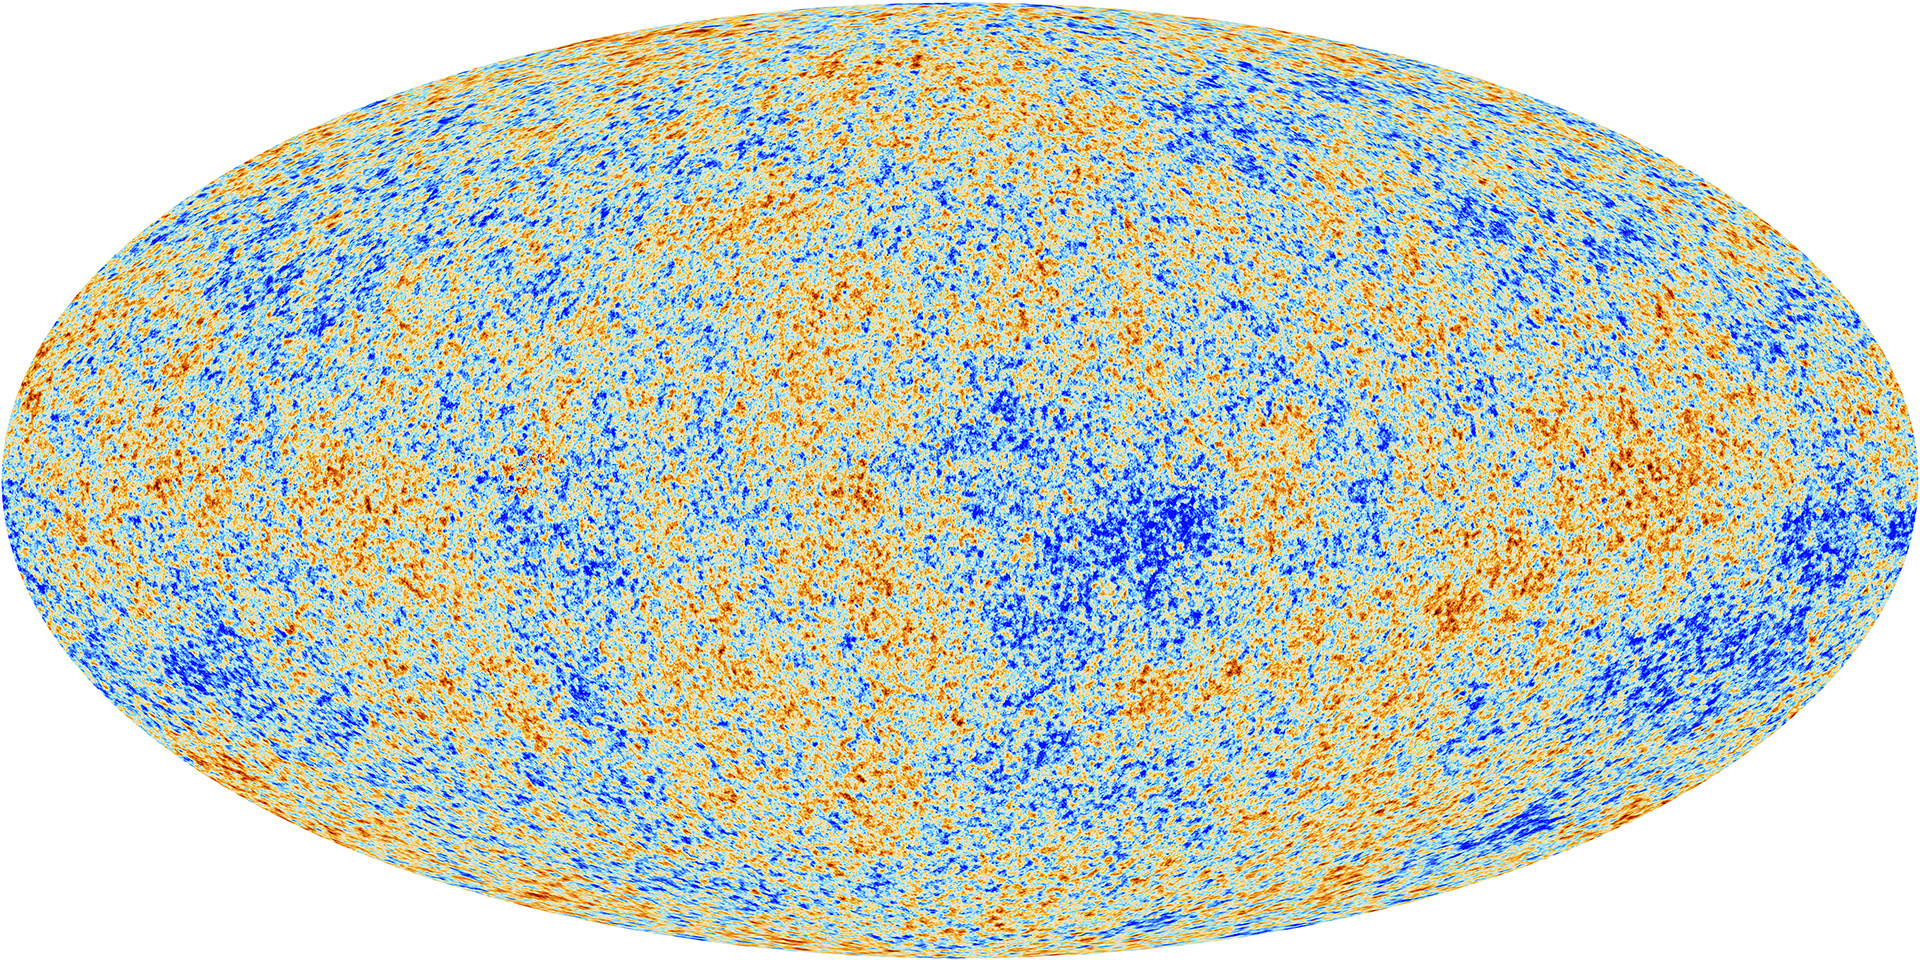
\includegraphics[height=.95\textheight]{img/01/CMB.jpeg} 
        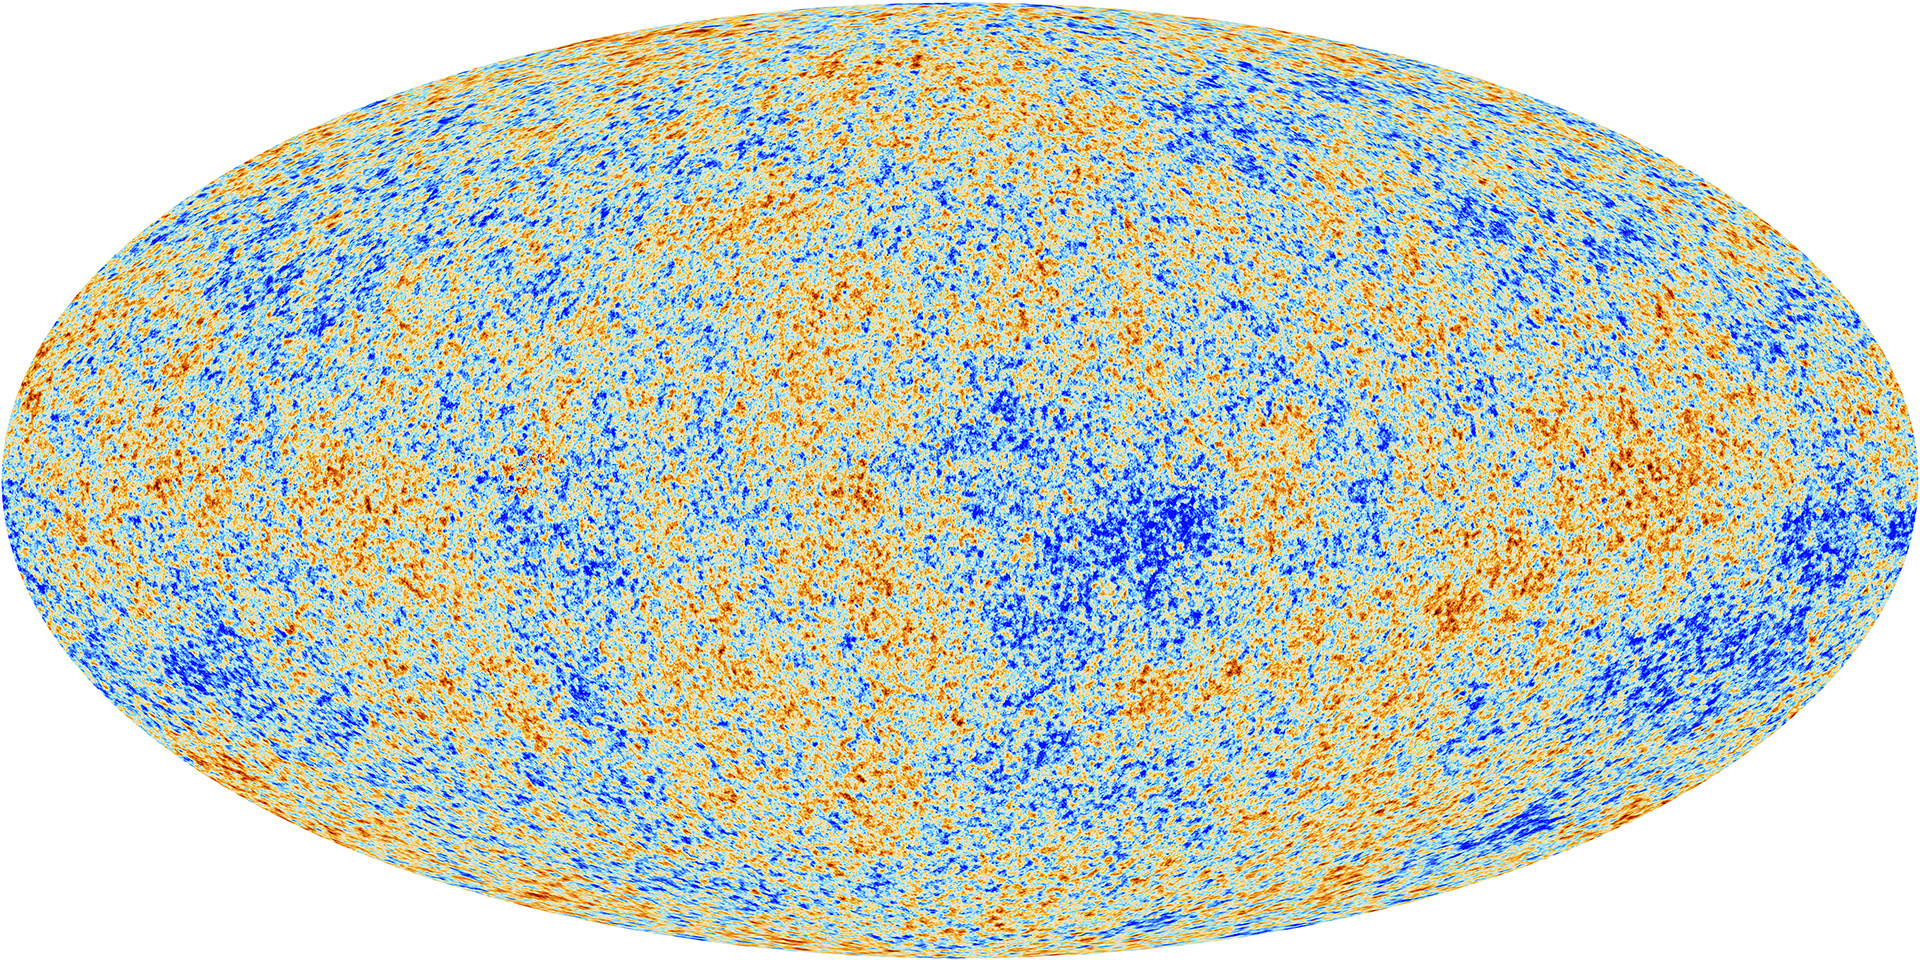
\includegraphics[width=0.95 \textwidth]{img/01/CMB.jpeg} 

        \caption[CMB]{Les fluctuations du \ac{CMB} vues par le satellite Planck. 
        Image ESA}
 		\label{fig:cmb}
\end{figure}

%Les anisotropies du \ac{CMB} sont étudiées en décomposant les fluctuations relatives de température en harmoniques sphériques.
%Un spectre de puissance, correspondant à la transformée de Fourrier de sa fonction de corrélation a deux points, caractéristique est obtenu (cf figure \ref{fig:cmb_power_spectrum}).

%%decomposition en multipoles
%%https://www.physicsforums.com/threads/can-someone-explain-angular-power-spectrum.309483/
%\begin{equation}
% \frac{\Delta T(\theta,\phi)}{T} = \sum_{l>0} \sum_{m=-l}^l a_{lm} Y(\theta,\phi)_{lm}
%\end{equation}
%
%avec : 
%
%\begin{equation}
%a_{lm}= \int d\Omega(\theta,\phi) \Delta T (\theta,\phi) Y(\theta,\phi)_{lm}
%\end{equation}
%
%%Fig\,\ref{fig:harmoniques_spheriques}
%%\begin{figure}[bth]
%%        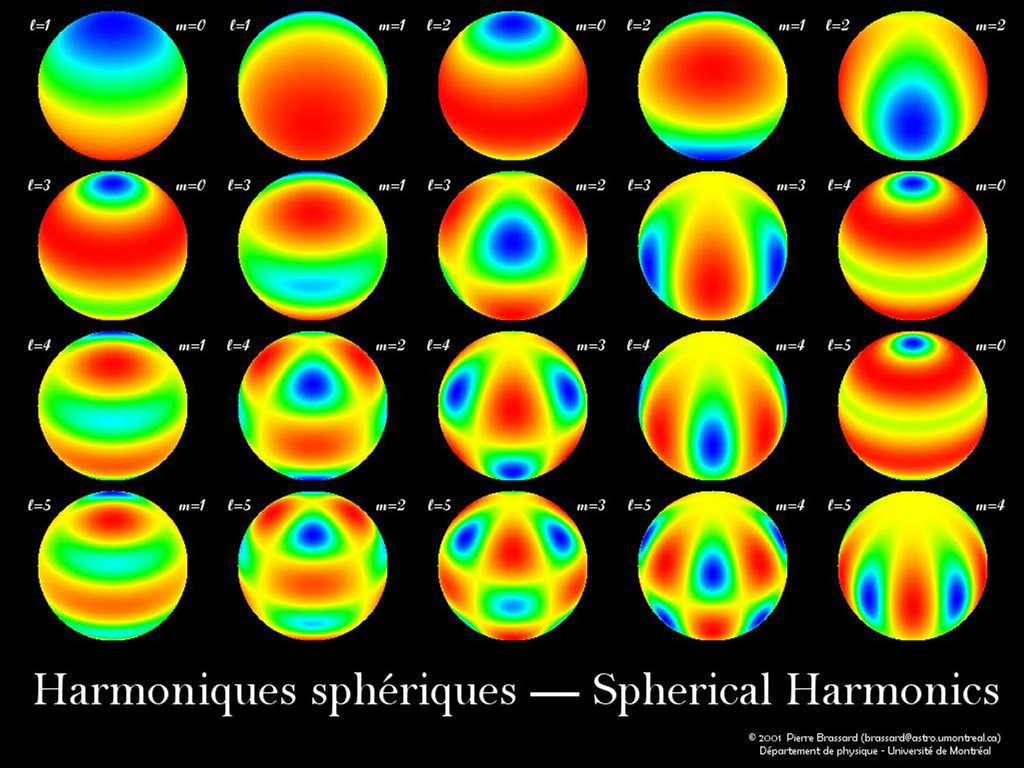
\includegraphics[width=.95\linewidth]{img/01/harmoniques_spheriques.jpeg} 
%%        \caption{
%%        représentation des $Y(\theta,\phi)_{lm}$
%% Pierre Brassard, université de Montréal 
%%%Spectre thermique du CMB vue par le satellite Cosmic Background Explorer (COBE). 
%%        Image Wikipédia}
%% 		\label{fig:harmoniques_spheriques}
%%\end{figure}
%
%\begin{equation}
%C_l = \frac{1}{2l+1} \sum_{m=-l}^l a_{lm} a_{lm}^*
%\end{equation}
%
%Et finalement, on obtient le spectre de puissance représenté Fig.\,\ref{fig:cmb_power_spectrum}:
%
%\begin{equation}
%D_l = \frac{l (l+1) C_l }{2 \pi} 
%\end{equation}


\begin{figure}
        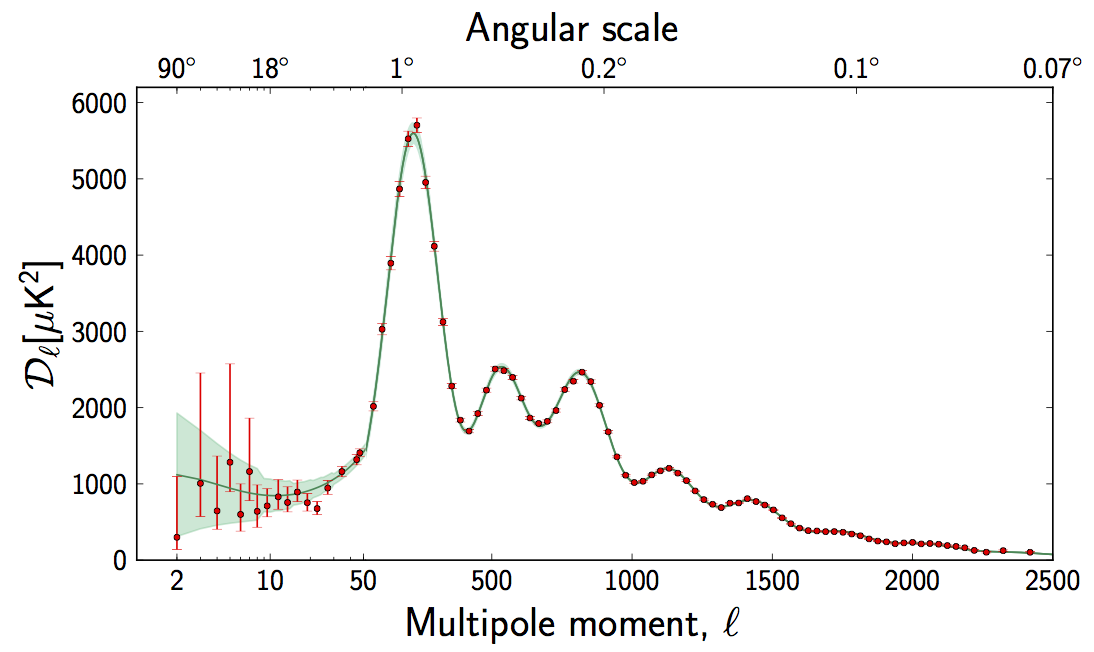
\includegraphics[width=.95\linewidth]{img/01/CMB_power_spectrum.png} 
        \caption[Spectre de puissance des fluctuation du CMB]{Spectre de puissance des fluctuation du \ac{CMB}.
        Image ESA}
 		\label{fig:cmb_power_spectrum}
\end{figure}

%Fig. \ref{fig:cmb_power_spectrum}

Le spectre de puissance du \ac{CMB} contient de l'information sur la distribution de la matière au moment de son l'émission, et ces fluctuations de température sont essentielles pour expliquer la formation des grandes structures observées aujourd'hui.
%En effet, comme il existe un lien direct entre la température et la densité, il est possible de déterminer la distribution de matière à l'époque de l'émission de \ac{CMB}.
%les régions aillant une température légèrement plus élevées correspondent aux régions légèrement plus denses, et réciproquement. 
%Nous verrons plus tard (cf section \ref{sec:IC}) que cette distribution de matière à très haut redshift permet la génération des conditions initiales nécessaire pour effectuer des simulations.

\section{Le contenu de l'Univers}
\label{cosmoparam}

\begin{figure}
        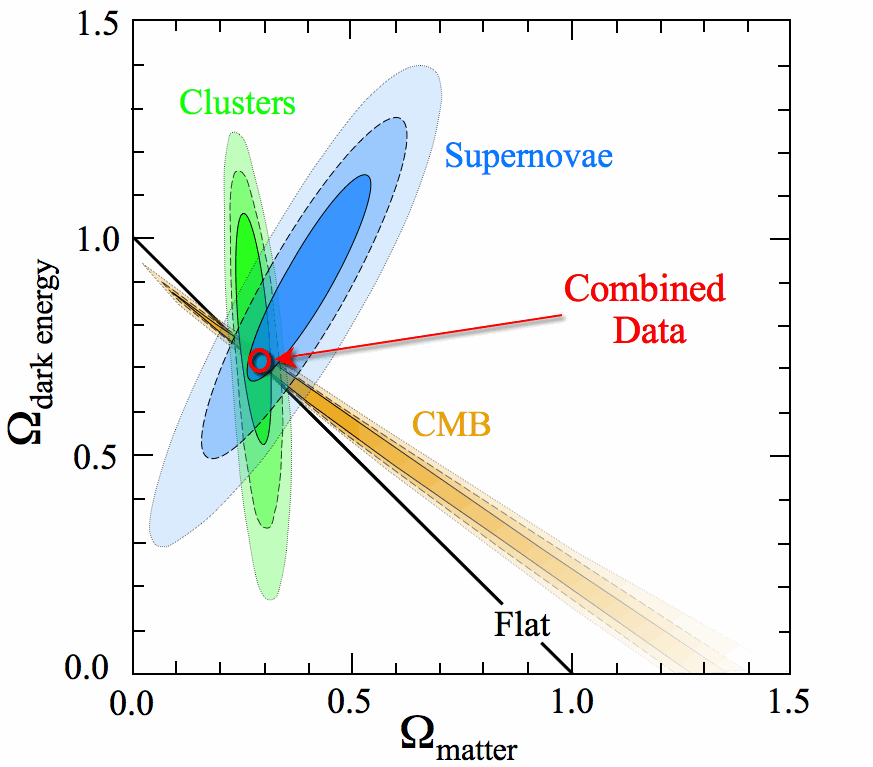
\includegraphics[width=.95\linewidth]{img/01/cosmoparam.png} 
        \caption[Determination des paramètres cosmologique]{Détermination des paramètres cosmologique a partir de différents observables. Figure extraite de \cite{2008ApJ...686..749K}}
 		\label{fig:cosmoparam}
\end{figure}


%La distribution des fluctuations de densité n'est pas la seule information contenue dans le \ac{CMB}, nous verrons dans la prochaine section que se spectre contient également de l'information sur l'abondance des différents constituants de l'Univers.
%La première étape pour comprendre l'univers, est de déterminer ce qu'il contient, et quelles sont les physiques dominante à considérer, en fonction de ce que l'on cherche à étudier.
Il est possible de créer un modèle théorique du plasma primordial et de l'utiliser pour prédire le spectre de puissance de l'émission de recombinaison.
En comparant le spectre de puissance théorique obtenu à celui du \ac{CMB} observé, il est possible de déterminer les paramètres libres du modèle cosmologique par ajustement.
La figure \ref{fig:cmb_power_spectrum} représente la comparaison entre le meilleur ajustement actuel et les observations.

La détermination des paramètres utilise conjointement plusieurs observables.
%Chacune de ces observables va pouvoir être lier à un modèle disposant de plusieurs paramètres libres.
Les supernovæ considérées comme chandelles standards, suffisamment lointaines permettent d'obtenir de l'information sur l'accélération de l'expansion de l'Univers.
% (un gamme de valeurs pour $\Omega_\Lambda$) (voir par exemple \cite{1999ApJ...517..565P} pour plus d'informations sur le sujet).
%Ou encore la distribution actuelles des galaxies, en partie reliquat des oscillations acoustiques dans le plasma primordial, permet de contraindre les paramètres cosmologique.
Ou encore l'abondance observée des amas de galaxies permettent de contraindre $\Omega_m$.

%A partir de différents observables,
%En recoupant les données obtenues a partir d'observations comme , 

%Le spectre de puissance du fond diffus cosmologique permet de déterminer les quantité respectives des différents constituants de l'univers.
%En recoupant ces données a d'autre observables, comme la distribution des amas de galaxies ou les supernovae lointaines, il est possible de contraindre les paramètres cosmologiques (Fig. \ref{fig:cosmoparam}).

Une représentation de ces différentes contraintes sur les paramètres de densité d'énergie noire et de matière est visible sur la figure \ref{fig:cosmoparam}.
Ces paramètres de densités ne sont pas les seuls paramètre libres du modèle standard et une compilation de ces paramètres est présentée sur la figure \ref{fig:planck_parameters}.
Ces paramètres ont été obtenus par \cite{planck_collaboration_planck_2016} et sont actuellement les plus récents disponibles.

%A partir du spectre de puissance, on peut déterminer les différentes composantes de l'univers (paramètres cosmologique).
%univers infini, homogène, isotrope


%https://ned.ipac.caltech.edu/level5/Freedman2/Freed6.html


\begin{figure}
        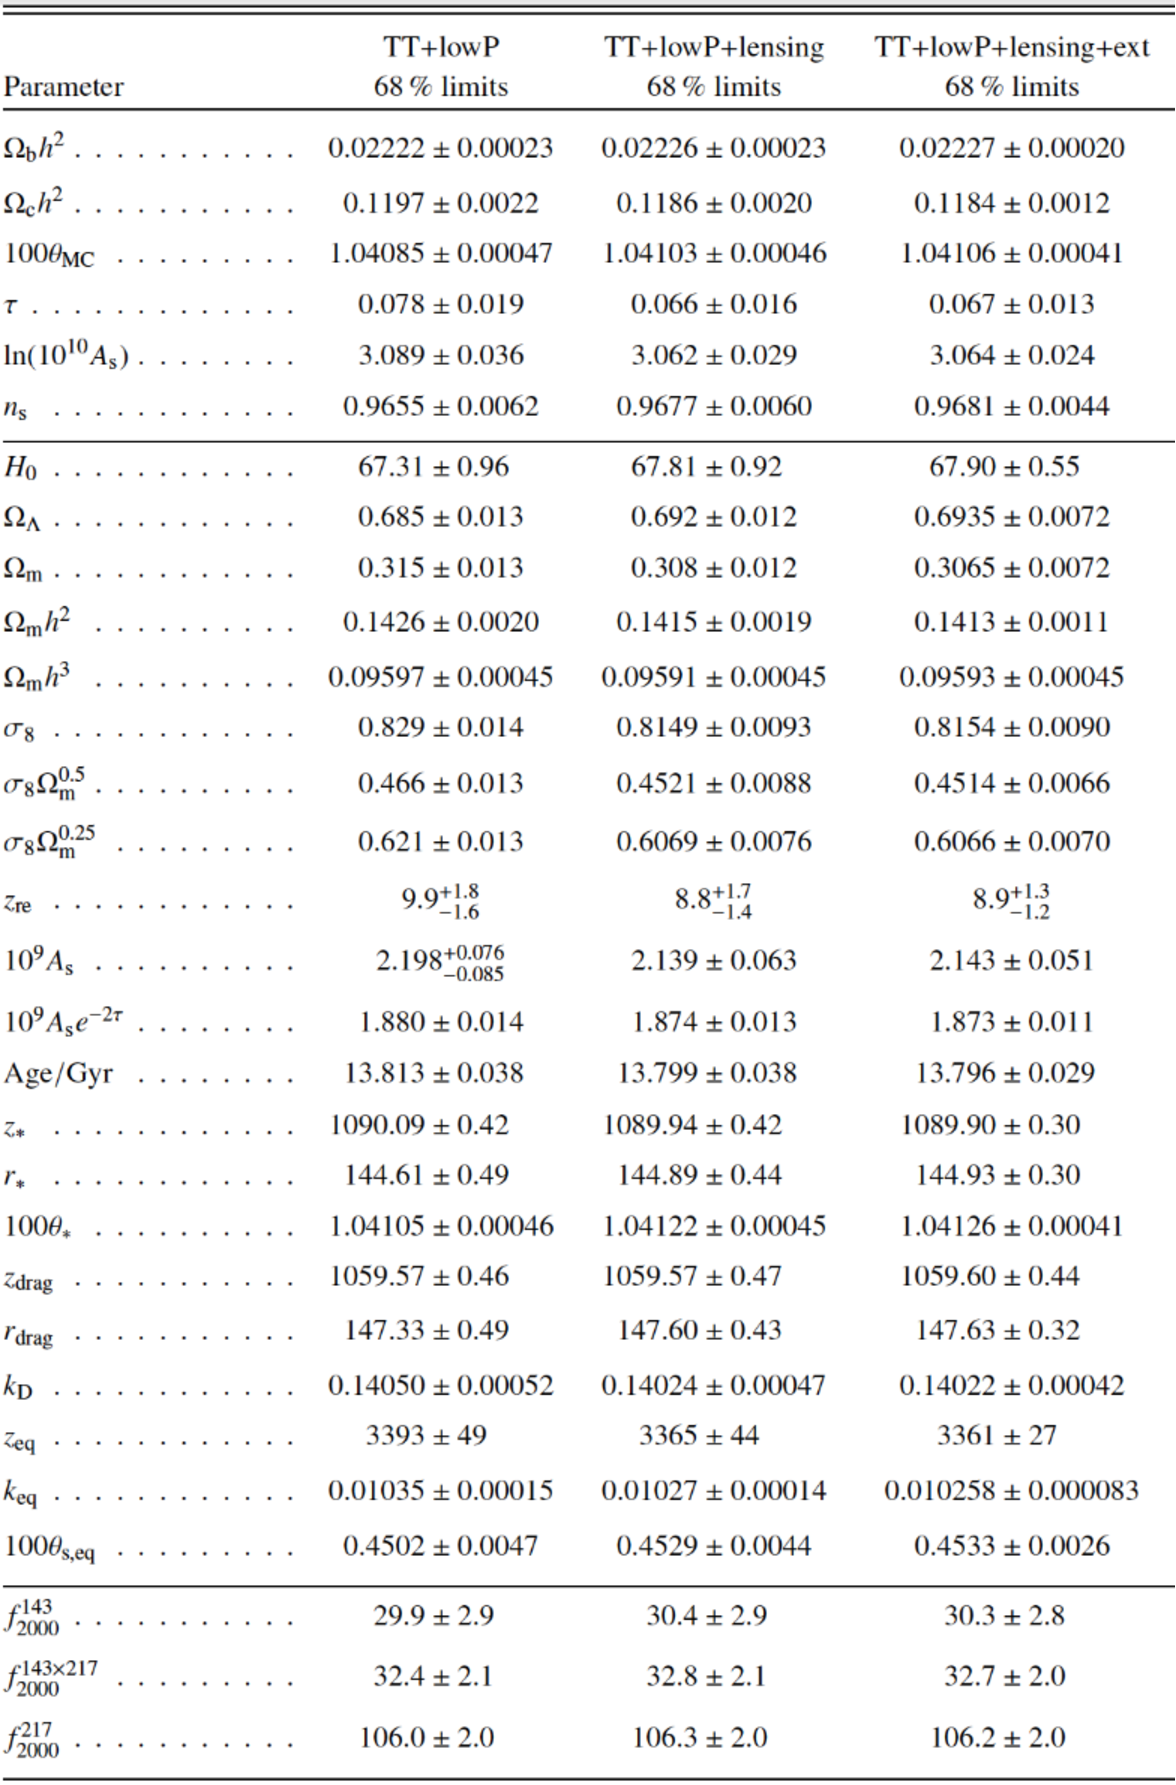
\includegraphics[width=.95\linewidth]{img/01/table_planck2.pdf} 
        \caption[Tables paramètres cosmologique]{Détermination des paramètres cosmologiques par \cite{planck_collaboration_planck_2016} }
 		\label{fig:planck_parameters}
\end{figure}
%
%
%
%\subsection{Énergie noire}
%Nous avons déjà abordé le sujet de l'énergie noire dans la section \ref{sec:dark_egy}.
%Avec une abondance relative de près de 70 \%, l'énergie noire est le principal constituant de l'Univers.
%Elle a été introduite pour expliquer l'accélération de l'expansion l'Univers.
%Elle contraint la distribution de matière sur les plus grandes échelles (de l'ordre du Giga parsec).
%Nous n'avons pas d'idée sur sa provenance mais des future missions comme EUCLID \citep{2016PhRvD..94l3515T} permettront d'obtenir plus d'information à son sujet.
%
%\subsection{Matière noire CDM}
%
%La matière noire est un vaste sujet.
%Le modèle $\Lambda$CDM nécessite une certaine quantité de matière pour expliquer les interactions gravitationnelles observées.
%Cette quantité de matière n'est pas en accord avec les observations réalisées sur la matière visible.
%Il a donc été nécessaire d’introduire une matière invisible appelée matière noire.
%La matière noire représente 26\% du bilan énergétique total et gouverne les échelles de l'ordre du Mega parsec.
%Elle est la principale source de gravitation et présente des propriétés non collisionnelles.
%
%Entre autres indications de la présence d'une matière non détectée, il y a:
%\begin{itemize}
%
%\item Les courbes de rotation des galaxies.
%Il est possible d’estimer la masse d'une galaxie à partir de sa luminosité (masse lumineuse).
%Il est également possible de déterminer sa masse en étudiant sa vitesse de rotation en fonction de son rayon (masse dynamique).
%La comparaison entre la masse dynamique et la masse lumineuse montre que les galaxies tournent plus vites que prévu et que la masse lumineuse est plus faible que la masse dynamique.
%
%\item Le bullet cluster.
%Il s'agit de la collision entre deux amas de galaxies dont les caractéristiques semblent actuellement présenter la meilleur piste en faveur de la présence de matière noire.
%
%\item Le spectre de puissance du \ac{CMB} (voir section \ref{sec:cmb_power_spectrum}), et plus particulièrement son troisième pic, est sensible au ratio matière/rayonnement et indique la présence de matière noire.
%
%\end{itemize}
%
%%\subsubsection{CMB}
%
%
%%\subsubsection{Bullet cluster}
%
%%echelle mega parsec\\
%%gouverne la gravité\\
%%non collisionnelle\\
%%
%%
%%\begin{figure}[bth]
%%        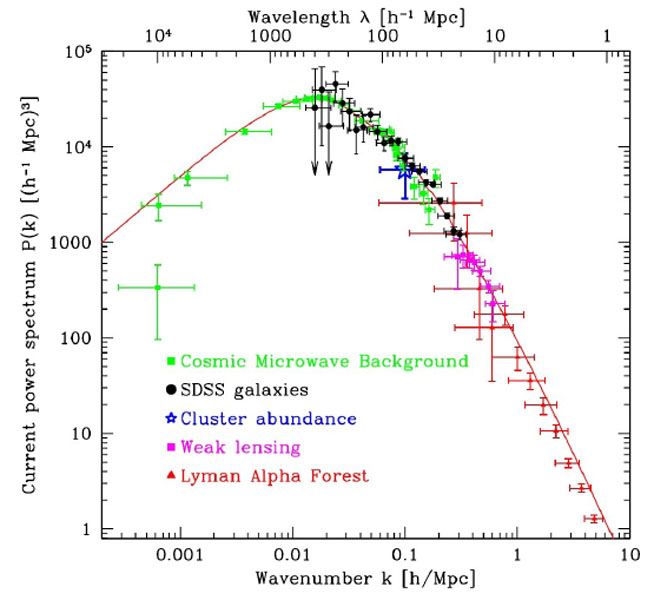
\includegraphics[width=.95\linewidth]{img/01/matter_power_spectrum.jpeg} 
%%        \caption{Spectre de puissance de distribution de la matière a grande échelle
%%        %http://adsabs.harvard.edu/cgi-bin/bib_query?2004PhRvD..69j3501T
%%        }
%% 		\label{fig:matter_power_spectrum}
%%\end{figure}
%
%\subsection{Baryon}
%
%Les baryons correspondent à la matière connue, avec laquelle la lumière interagis.
%Ils ne représentent qu'environ 5\% du bilan énergétique global.
%Les baryons interagissent également entre eux, et ont une physique collisionnelle.
%Leur introduction dans les simulations a été nécessaire lorsque l'on a commencer à étudier des échelles de l'ordre du kiloparsec et la formation stellaire.
%
%%echelle kilo parsec
%%collisionnelle
%%interagit avec la radiation
%%La matière visible
%
%\subsection{Radiation}
%
%La radiation ne représente aujourd'hui que $10^{-4}$ de l'énergie totale.
%Elle représente notre seul source d'information sur l'univers (Ce n'est plus le cas depuis la récente découverte des ondes gravitationnelles) %TODO ref
%Elle est centrale dans le processus de réionisation.
%La radiation est capable d'impacter a la fois les petites échelles de l'ordre du parsec (en interagissant avec la formation stellaire)
%et aux grandes échelles de l'ordre de la centaine de Méga parsec en changeant les propriétés optiques de l'\ac{IGM}.
%
%%A la fois les grandes échelles et les petites.
%%Son introduction dans les simulations 
%
%%seulement E>13.6 eV
%
%
%%\subsection{Bilan}
%%
%%plot en camembert avec les différents constituants
%
%%perturbation lineaires:
%%https://ned.ipac.caltech.edu/level5/Sept11/Norman/Norman2.html


\section{Formation des structures}
\label{sec:formationgalaxie}

%Nous avons vu dans la partie dédiée au fond diffus cosmologique que  
L'Univers n'était pas parfaitement homogène lors de l'émission du \ac{CMB} et la croissance des perturbations primordiales va mener, sous l'effet de la lutte entre l'expansion et la gravitation, à un effondrement de la matière sur elle même \citep{1968ApJ...151..459S}.
%C'est dans ces surdensités locales que vont se former les premières galaxies.
La première étape à la formation d'une galaxie est donc l'effondrement d'une surdensité et cet effondrement est largement dominé par la matière noire \citep{1985ApJ...292..371D}.

Pour étudier la croissance des fluctuations primordiales dans le régime linéaire on utilisera la théorie des perturbations et on remplacera la densité par la densité perturbée $\rho(x) = <\rho> + \delta(x)$ où $\delta$ sera appelé le contraste de densité :

\begin{equation}
\delta(x) = \frac{\rho(x)}{<\rho>} -1.
\end{equation}

On cherchera alors une solution des équations régissant le fluide primordial, en utilisant l'approximation au premier ordre \citep{1999coph.book.....P}.
Cette approche permet de prédire les oscillations acoustiques des baryons ou Baryonic Acoustic Oscillations (BAO) observées dans la distribution des galaxies \citep{2005ApJ...633..560E}.
Pour rester dans le domaine linéaire, le contraste doit rester faible et représenter l'homogénéité de l'Univers aux grandes échelles.

%A partir de cette solution perturbée, \cite{1970A&A.....5...84Z} propose une approche dynamique (voir \cite{2014MNRAS.439.3630W} pour une revue récente) permettant la génération de conditions initiales utilisées dans les simulations numériques.
%En effet, 
Arrivé à la fin du régime linéaire, il devient nécessaire d'utiliser des simulations numériques pour étudier la formation des structures en détails.
Les simulations de croissances des structures réalisées avec les considérations exposées dans cette section donnent une excellente similarité avec les observations (voir figure \ref{fig:sdss}).

\begin{figure}
        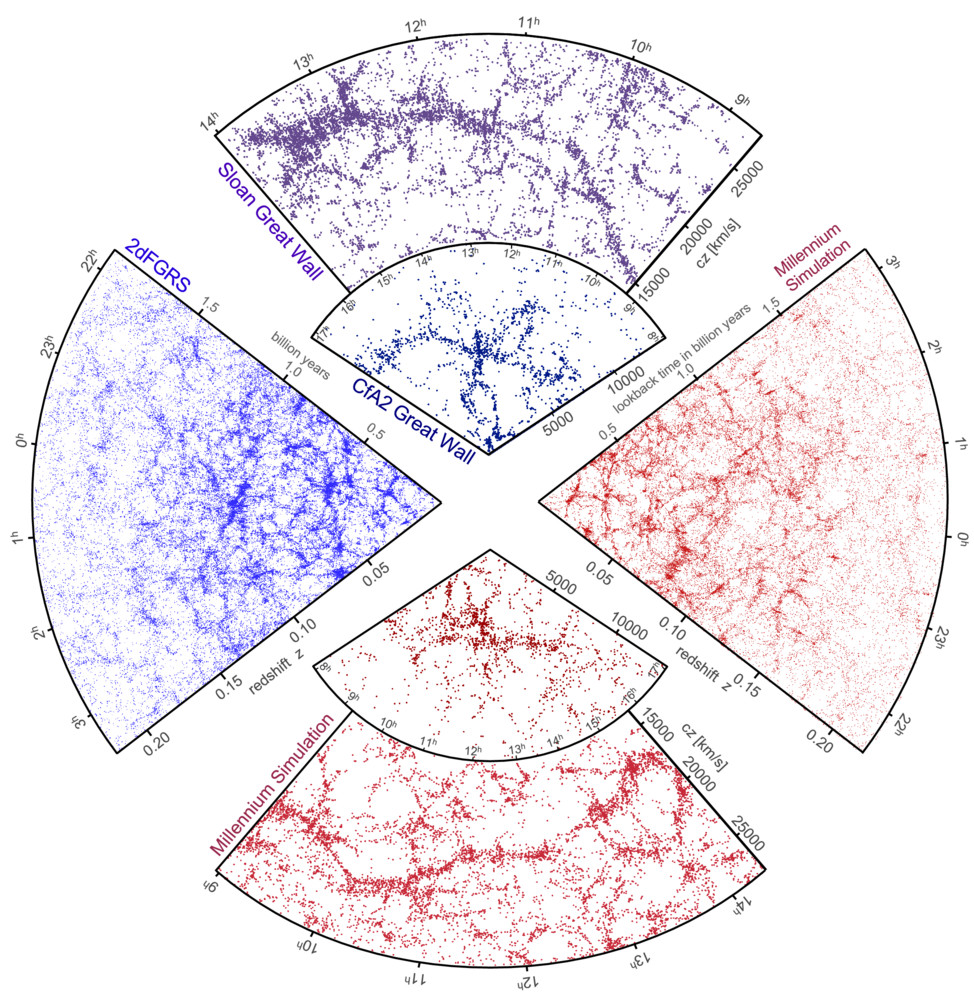
\includegraphics[width=.95\linewidth]{img/02/sdss_millenium.jpeg} 
        \caption[SDSS - Millennium]{Comparaison entre les structures à grandes échelles observées par le SDSS (en bleu) et celles reproduite dans la simulation Millennium \citep{2005Natur.435..629S} (en rouge).
%http://wwwmpa.mpa-garching.mpg.de/millennium/
 		\label{fig:sdss}}
\end{figure}

Malgré la forte non-linéarité de la croissance des structures, il est tout de même possible de faire quelques prescriptions analytiques.
Notamment en considérant le cas idéal de l'effondrement d'une surdensité sphérique dans le cas d'un Univers en expansion.
En cherchant les solutions de:
\begin{equation}
\frac{d^2r}{dt^2} = -\frac{GM}{r^2} + \frac{\Lambda}{3}r, 
\end{equation}
ou $M$ est la masse contenue au sein d'une coquille sphérique de rayon $r$, et en y appliquant le théorème du Viriel:
\begin{equation}
2T+U=0
\end{equation}
où $T$ est l'énergie cinétique et $U$ l'énergie interne, il est possible de déterminer $\Delta_{vir}$ la densité moyenne des structure en effondrement \citep{2010gfe..book.....M}.
Dans le cas d'un Univers plat cette surdensité s'exprime :
\begin{equation}
\Delta_{vir} \approx (18 \pi ^2 + 82 (\Omega_m-1) - 39 (\Omega_m-1)^2)/ \Omega_m
\end{equation}

En pratique $\Delta_{vir}$ est de l'ordre de $\approx 200 \bar{\rho}$.
Dans la suite on considérera $R_{200}$ le rayon d'une surdensité de $200 \bar{\rho}$ comme une approximation du rayon de Viriel $R_{vir}$:
\begin{equation}
R_{200} \approx R_{vir}
\end{equation}

Cet effondrement va mener à la formation de structures majoritairement composée de matière noire.
Ces halos de matière noire vont former des puits de potentiel et entraîner les baryons qui formerons les galaxies.

Pour qu'une surdensité s'effondre, il faut que sa masse soit supérieure à la masse de Jeans.
Après le découplage matière/rayonnement cette masse chute brutalement \citep{2010gfe..book.....M}, autorisant la contraction de structures de $M \approx 10^6 M_\odot$.
Cette masse évolue en fonction du redshift \citep{2016PhR...645....1B} : 
\begin{equation}
M_j \approx 6 \cdot 10 ^3 \left( \frac{1+z}{10} \right)^{3/2} M_\odot
\end{equation}

Ces halos auront différentes masses en fonction des fluctuations de densités initiales.
On définis le spectre de puissance des fluctuation de densité comme :

\begin{equation}
P(k) = \left< | \delta(x) |^2 \right>
\end{equation}

En analysant la variance de $P(k)$, \cite{1974ApJ...187..425P} ont déterminé $n$ le nombre halos ayant une masse comprissent en $M$ et $M+dM$
\begin{equation}
\frac{dn_{(M,t)}}{dM} = \sqrt{\frac{2}{\pi}} \left| \frac{\rho_0}{M^2} \right| \frac{d ln \sigma}{d ln M} \frac{\delta_0}{\sigma_{(M)}} exp \left[ - \frac{\delta_{0c}^2}{2\sigma_{(M)}^2} \right].
\end{equation}

Cette grandeur est appelée fonction de masse des halos ou \ac{HMF} et est représentée sur la figure \ref{fig:hmfpress}.
Depuis d'autres formulations ont été introduites (eg \cite{1999MNRAS.308..119S}).

\begin{figure}
        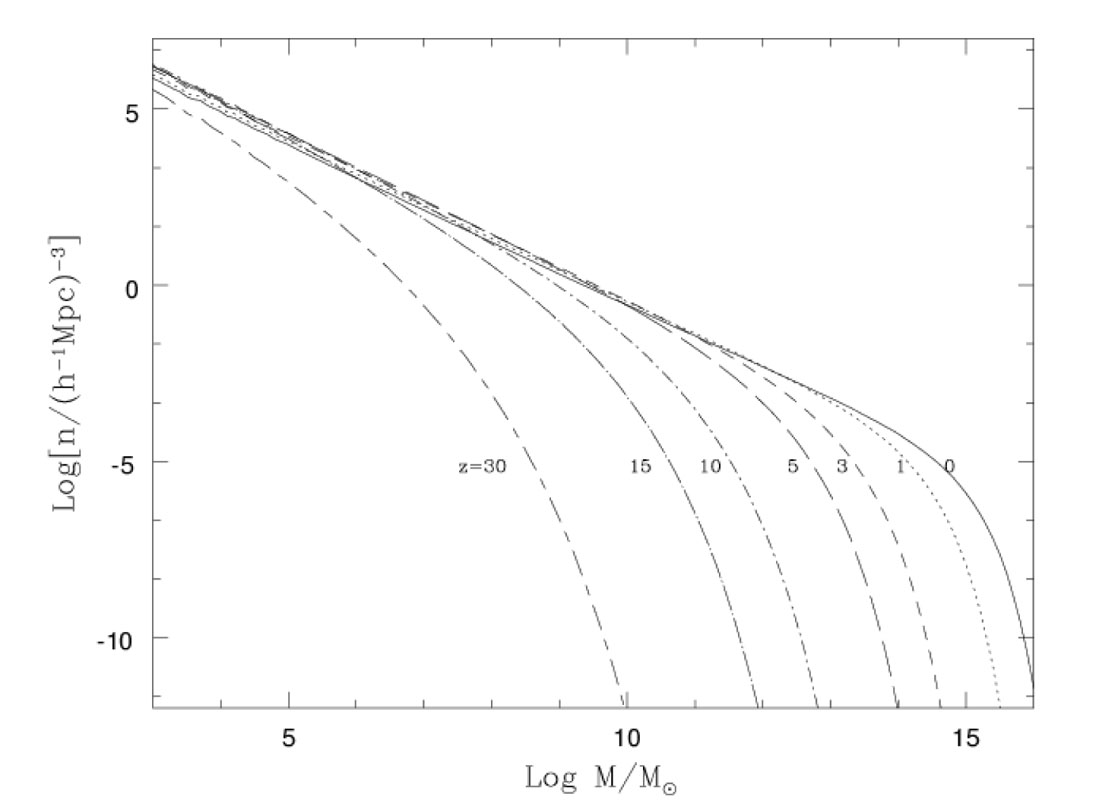
\includegraphics[width=.95\linewidth]{img/01/press.jpg} 
        \caption[HMF théorique]{Fonctions de masses théoriques de halos déterminées par \cite{1974ApJ...187..425P} à différents redshifts.
        Image issue de \href{ned.ipac.caltech.edu}{ned.ipac.caltech.edu}
 		\label{fig:hmfpress}}
\end{figure}
